\subsection{The Gandalf Framework}
The amplified and shaped output signal of the \ac{emusic} \ac{asic} needs to be digitized.
This step is done by Gandalf modules.
Originally developed at the University of Freiburg for the \ac{compass} experiment it has a modular design to fill different roles in the experiments \ac{daq}.
Using mezzanin cards different signal, clock and trigger inputs can be chosen.
In the following the Gandalf framework will be introduced.
The mezzanin cards not used in this work are therefore only mentioned but not presented in detail.
A overview of a Gandalf module is shown in \autoref{fig:gandalf_overview}.
\begin{figure}
	\centering
	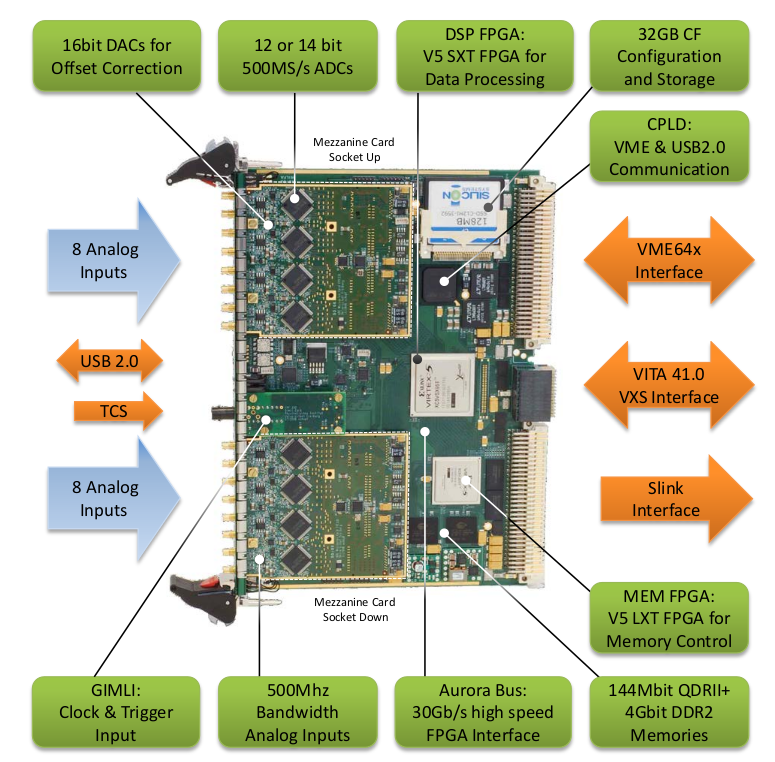
\includegraphics[width=1.\linewidth]{pictures/gandalf_overview.png}
	\label{fig:gandalf_overview}
	\caption{Overview of the Gandalf module equiped with Analog Mezzanin Cards (AMCs) and the fiber Gimli mezzanin card for clock an trigger input. The analog waveforms are digitized by the AMCs and the digitized data is processed by the DSP FPGA. The MEM FPGA handles the memory of the processed data, which can be transfered to a computer via the USB inteface on the front of the VME or S-Link interfaces on the backplane. \cite{herrmann}}
\end{figure}

\subsubsection{Input Mezzanin Cards}
The Gandalf module has two mezzanin card slots for input signals.
For these slots three different mezzanine cards were developed, \ac{amc}, \ac{dmc} and \ac{omc}.

